%%%%%%%%%%%%%%%%%%%%%%%%%%%%%%%%%%%%%%%%%%
\chapter{Introduction} \label{sec:introduction}
%%%%%%%%%%%%%%%%%%%%%%%%%%%%%%%%%%%%%%%%%%
% brief intro of pebble beds
Helium-cooled pebble beds (HCPB) of lithium ceramics are candidate designs in many current nuclear fusion demonstration reactors as well as tritium breeding modules to be tested in the ITER experiment. The HCPBs will endure large neutron fluxes in order to generate both the heat for electricity production as well as tritium for a self-sustained fuel cycle. There are many features of the HCPBs that make thermal characterization important and complicated. Firstly, the heat generated in the ceramic pebbles from the neutrons is transported into the structural material containing the pebble bed, then into a coolant (generally high-pressure helium) running through channels in the containing structure. Therefore maintaining contact between the granular material and the structural material is necessary to allow the flow of heat out of the pebble bed and into the coolant. Secondly, tritium release in the ceramic pebbles is a strong function of temperature which imposes a minimum operating temperature of the pebble beds. Simultaneously, a maximum operable temperature of the pebble beds is enforced to avoid widespread sintering of the ceramic materials which would also increase tritium retention in the solid pebbles. Thus the HCPBs have relatively narrow operational temperature window that is dependent, in part, on maintaining good mechanical contact with its structural container. Understanding pebble bed interactions with its container is therefore necessary to gain temperature prediction and control which is of utmost importance for desirable tritium release and energy production of a HCPB in a fusion reactor.

In spite of the many engineering applications of granular materials, the physical origins of heat transfer mechanisms in packed beds are still not thoroughly understood nor characterized. Many experiments in engineering and fusion communities have been carried out with the goal of treating the granular bed as a fictitious continuous media and then developing phenomenological models for effective material properties. In this approach, heat transport in pebble beds is often characterized with an effective thermal conductivity, $\keff$. Many models have shown their ability to accurately predict the temperature profiles for pebble beds under similar operating conditions to the beds for which the models were developed. However, the accuracy of the model predictions often degrade as soon as a pebble bed's granular material, grain radii distributions, or operating conditions vary from the experimentally studied packed beds. In addition, the ceramic materials chosen for use in HCPBs (\textit{e.g.} \lit and \lis) have shown a propensity for creep, crushing, and inter-particle sintering which alter the morphological structure of packed beds in ways not currently predictable with the effective material characterizations. Moreover, effective conductivity models have been developed with the consideration of stagnant interstitial fluid which is insufficient to capture the thermal influence of the helium purge gas flowing through the ceramic pebble beds in fusion reactors.

To overcome the limitations of empirical observations of effective material properties, and aided by the acceleration and availability of computational power, researchers have shifted their attention to studies of the interacting physics on the grain-scale. The discrete element method (DEM) has emerged as an extremely powerful approach for interrogating and modeling the evolving transient grain-scale information in packed beds. DEM models have also been shown to be effectively coupled to volume-averaged computational fluid dynamics (CFD) models. Coupled CFD-DEM models are capable of predicting temperature distributions in ceramic pebble beds with the slow-flowing interstitial purge gas while continuing to provide useful information on grain-scale interactions: contact forces leading to single grain crushing, resettling of the pebble bed, and the ability to remove nuclear heat deposition to the coolant in the containing structure.


The science and modeling of granular materials has a long and rich history. Coulomb proposed ideas of static friction in 1773, Faraday in 1831 discovered the convective movement of powders, and even Reynolds in 1885 introduced notions on granular expansion and shear.\cite{Jaeger1996a} Yet despite the diverse fields interested in granular materials, the description of them with classic continuum mechanics is still far from complete; quite different from the conclusively described constitutive equations of elastic theory, hydrodynamics, and gas dynamics that have existed for two centuries.\cite{Sadovskaya2012} Granular materials play in important role in civil, geotechnical, chemical, and mechanical engineering in industries as diverse as pharmacy, automative, agriculture, and construction to name just a few.\cite{Hill} A resurgence of interest in granular materials has also happened in the fields of applied mathematics and physics as metaphors for other dynamical systems.\cite{Jaeger1996a}

Even if we restrict our consideration to static packings of non-cohesive granular materials (neglecting the complex, unusual granular hydro- and gas dynamics), modeling is complicated by the heterogeneity of contact forces running through the packed grains and the packing structure of the grains.  The granular medium introduces complexity to modeling, in part, due to its significant different between compression and tension experiments; under compression the granular medium behaves as if an elastic or elasto-plastic body but offers no resistance to tension. Furthermore, when an external excitation such as vibration is introduced into the metastable packing state of a granular system, the packing is unlocked to slowly travel through packing phase space at a logarithmically slow pace[barker and mehta 1993, mehta 1994, knight 1995] Nonetheless, many material models have been developed in an attempt to describe the mechanics of a granular system as a fictitious continuum with varying success and applicability.

Mechanics described by drucker & prager[cite drucker and prager, etc. see \cite{Hill}]. The heat transfer in granular materials also done on a continuum [zehner shlunder, van antwerpen, etc.]. 

In 1979, Cundall \& Strack opened a new avenue for studying granular materials when they introduced the distinct element method (later renamed by the community as the \textit{discrete} element method).\cite{Cundall1979} Since then, grain-scale descriptions of granular systems have taken prominence for their ability to enrich the macrosopic models when they are insufficient to describe the rheology of a granular material. In the approach of Cundall \& Strack, all of the individual grains in a system are described as rigid elements for which the equations of motion can each be simultaneously integrated based on the (typically localized) interacting forces.

Granular system became important to fusion power reactors after the introduction of a solid, non-mobile tritium breeding blanket design by by Abdou\etal\cite{Abdou1975} in 1975, the so-called `solid breeder' or `ceramic breeder' beds of lithium ceramics. In a a solid breeder a packed bed of grains (in this dissertation, a `grain' is also referred to simply as a particle or a pebble interchangeably) is in physical contact with a structural material and allows a purge flow of helium through the void space between grains. Neutrons are ejected from the burning plasma of the fusion reactor and collide with the lithium of the packed bed. The reaction deposits heat and transmutes the lithium into tritium -- which is collected in the purge helium for recycling as a fuel for the continued burn of plasma. The complex interactions of grains in this system is made even more so by the introduction of irradiation embrittling, heat generation and transport, and high-temperature material effects such as sintering and creep.

Because of the large size scale and complex interactive physics of solid breeders, it is desirable to employ the continuum-based models on the packed beds of ceramics with effective Thermomechanical properties derived from experiments on granular beds. However, current continuum models will be shown to be insufficient for capturing the evolving thermomechanics of the packed bed as bed resettling, individual grain crushing, and the helium purge influence the packing structure and inter-particle force networks in the bed. Thus in this dissertation I will approach the pebble bed from the microscopic scale of individual grains via the discrete element method to enable predictive capabilities for temperature profiles in ceramic breeder pebble beds with a helium purge gas -- even those experiencing bed resettling and grain crushing. Along the way, new constitutive relationships for material properties are discovered, fragmentation models are created, and new heat transfer models are incorporated.

In the rest of this chapter, I will introduce in more detail the necessity for thermal management in solid breeder designs and review the state-of-the-art in continuum modeling of solid breeders and their critical drawbacks both topics will act as motivation for the work presented in this dissertation. Then I will describe the objectives of my research and walk through the blueprint of satisfying them.


\begin{figure}[ht]
	\centering

	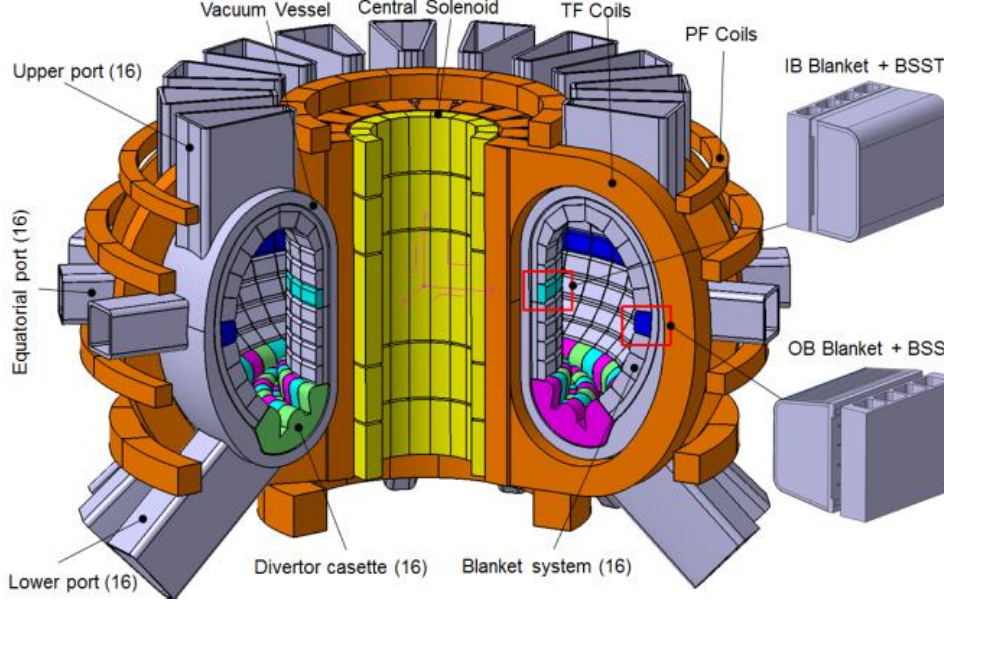
\includegraphics[width=\singleimagewidth]{chapters/figures/demo} 
	\caption{An example design of a DEMO reactor with solid breeder blankets shown as inboard (IB) and outboard (OB) blanket components.}
	\label{fig:demo}
\end{figure}

\begin{figure}[ht]
	\centering
	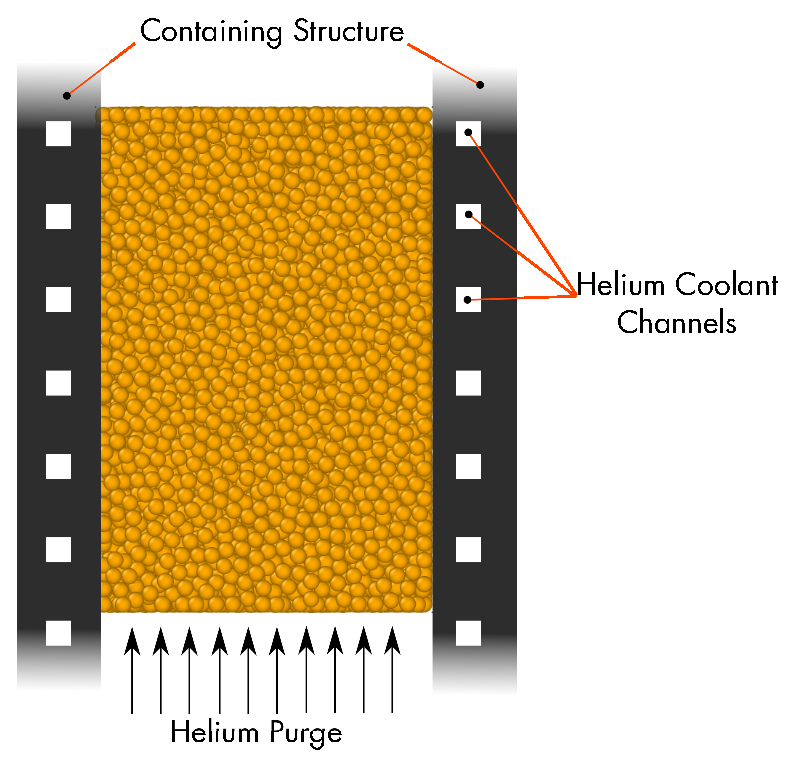
\includegraphics[width=\singleimagewidth]{figures/solid_breeder_sketch} 
	\caption{Sketch of a typical unit of a pebble bed tritium breeding zone. The pebble bed is cooled with contact to the containing structure.}
	\label{fig:solid-breeder-sketch}
\end{figure}

The breeder blanket is a critical piece of engineering technology upon which the success of a fusion power plant largely rests. The successful operation of a breeder will see the device capture the neutrons ejected from the fusion reaction to generate fuel for future reactions via the transmutation of lithium into tritium, act as shield to other sensitive equipment and personnel, and convert energy into extractable heat for electricity production. Figure~\ref{fig:demo} shows an example sketch of a demonstration (DEMO) fusion reactor and the relative location of the breeder blanket modules as they face the plasma in the torus of the tokamak. 



From the inception of the solid breeder concept, designs have evolved significantly in response to requirements of operation in the harsh fusion environment. Currently, the reference solid breeder design incorporates packed beds of ceramic pebbles (spherical particles) that are filled into containment structures of volumes optimized for thermophysical and tritium responses. The pebble bed form has ultimately become the design of choice based on many of its attractive features. Many requirements of a solid breeder `material' (the volume of a pebble bed is often considered as a single fictitious material) are satisfied by the ceramic pebble bed. The small pebbles provide a sufficient surface-area to volume ratio; have good and customizable (via polydispersity) open-porosity to allow the helium purge gas to wind through and pick up any generated tritium from the solid; and the small size of the pebbles prevent any large thermal gradients from emerging across any single solid material object -- thus increasing the mechanical survivability of the ceramic. 

[small paragraph describing a solid breeder such as EU's design]

\subsection{Solid Breeder Thermal Management and Temperature Window}
In Fig.~\ref{fig:solid-breeder-sketch}, a generic solid breeder volume is shown in order to point out major features of the pebble bed design. The pebble bed is contained by a low-activation steel which serves as both mechanical and thermal boundaries for the ensemble. The breeding blanket will experience high volumetric heating (resulting from secondary $\gamma$ rays and the kinetic energy of neutrons that are carrying away approximately 80\% of the fusion reaction) and temperatures will be allowed to increase to an allowable limit, $T_\text{max}$, which will be discussed in more detail shortly. The heat generated in the pebbles is transported through the bed volume through a number of paths, ultimately making its way into the containing structure and then into the high-pressure coolant.A high pressure (approximately 8 MPa) helium coolant is then run through the structure. The coolant will heat to approximately 500~\celsius~before exiting the blanket, maintaining the steel below structural temperature limits. The heat carried away by the coolant ultimately works its way into an electricity-producing cycle. 

 It is conducted via inter-particle contacts between pebbles, contact with the structural material, and convection to the purge gas then transported to the structural material. 

As the neutrons bombard the lithiated ceramic, tritium is produced internal to the pebbles. Tritium that transmutes from the lithium inside the pebble will diffuse slowly through the bulk until reaching a grain boundary. Tritium moves relatively quickly along the grain boundary until reaching a surface of open porosity where it may desorb into the passing purge gas.\cite{Federici1990} The low-pressure, low-speed purge gas is pumped through the pebble bed to extract the tritium generated and transport it out of the blanket for processing. 

The dual role of the breeding blanket to generate heat and tritium forces a specific operational temperature window for the ceramic pebble beds. The low end of the temperature window is governed by a minimum temperature for acceptable release rates of tritium from the ceramic to the purge gas; the value is generally set around 300~\celsius. Based on the current understanding of tritium release from the pebble, as grains grow during sintering of the ceramics the tritium release rate is expected to decrease beyond acceptable limits. Thus the upper limit of the temperature window is chosen to avoid sintering of the lithiated ceramic, giving the approximately 900~\celsius~limit mentioned previously. 

\begin{figure}
        \centering
        \begin{subfigure}[b]{\doubleimagewidth}
                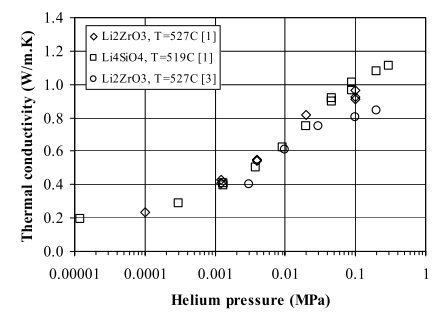
\includegraphics[width=\textwidth]{figures/keff-pressure}
                \caption{Effective conductivity of ceramic pebble beds is dependent on the pressure of the interstitial gas, a minimum of about $\keff = $\SI{0.2}{\watt\per\meter\per\kelvin} in vacuum.}
                \label{fig:keff-pressure}
        \end{subfigure}%
        
          %add desired spacing between images, e. g. ~, \quad, \qquad, \hfill etc.
          %(or a blank line to force the subfigure onto a new line)
        \begin{subfigure}[b]{\doubleimagewidth 	}
                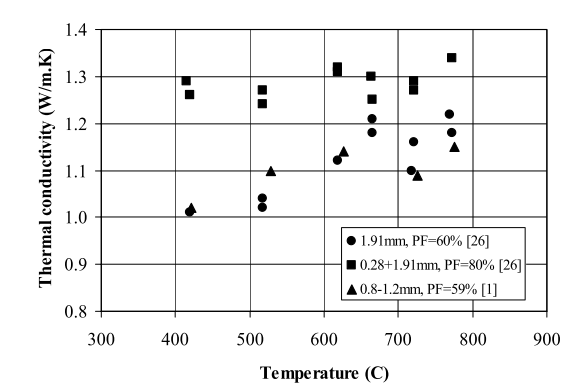
\includegraphics[width=\textwidth]{figures/lit-keff-exp}
                \caption{The effective conductivity of pebble beds is weakly dependent on external mechanical pressure and is always approximately $\keff = $\SI{1}{\watt\per\meter\kelvin} in helium.}
                \label{fig:keff-lit}
        \end{subfigure}
        \caption{Effective conductivity of lithium ceramics. Results from Ref.~\cite{Abou-Sena2005}}\label{fig:keff}
\end{figure}

Many experiments have been run to measure the effective thermal conductivity of a volume of ceramic pebbles. In Figs.~\ref{fig:keff}, the effective conductivity is seen to be strongly affected by the interstitial gas but weakly affected by the mechanical loads on the bed. The main conclusions to bear in mind from Fig.~\ref{fig:keff} are that: 1) the interstitial gas is an important transporter of heat in the bed and 2) the effective thermal conductivity of the pebble bed is low and will limit the size of the ceramic pebble bed volume to satisfy the temperature window mentioned above.

% The size of breeder region is limited by the operational temperature window that must be held in spite of the the poor effective conductivity of packed beds of ceramic pebbles. The conductivity is experimentally shown to be a weak function of external pressure but can generally no greater than about \si{1 W/{mK}} -- for well-packed beds. Because the effective conductivity and packed bed-wall interface conductance is predominately a contact conduction, disruptions to the packing structure will have considerable impact on the heat transfer of the packed bed.

As nuclear energy is deposited into the poorly-conductive ceramic breeder material and the temperature climbs well above the containing structure, the pebbles will each individually begin to grow from thermal expansion. The containing structure will confine the thermal expansion of the lithium ceramic and therefore lead to large mechanical stresses at the points of contact of the individual pebbles in the packed bed. As a ceramic material, the pebbles are prone to brittle failure when the contact forces grow large. But the ceramic pebble beds must be able to survive the high temperature, high stress, and irradiated environment while providing a reliable amount of tritium to the fuel processing equipment.

\subsection{Temperature Window for Ceramic Solid Breeders}


 % the fusion reaction deposits   The nuclear heat generated in the pebble bed solid breeder will heat the ceramic pebbles to maximum temperatures of approximately 900~\celsius. The heat of the pebbles is transported through them via conduction through inter-particle contacts, conduction through the purge gas into neighboring particles, and ultimately through contact with the containing structure. The box structure surrounding the solid breeder will have high pressure (\si{8~MPa} in many current designs) 


\section{Motivation}\label{sec:motivation}





\section{Objectives of this Study}\label{sec:intro-scope-of-work}
The goal of this work is to develop predictive capabilities for the onset and repercussions of pebble damage in an ensemble; to understand of the evolution of pebble bed morphology and thermophysical properties dependent upon the morphological state. The specific objectives of this dissertation are therefore to develop tools for modeling pebble interactions, predict pebble crushing based upon the mechanical interactions, and monitor the macroscopic changes to temperatures in the bed in response to damaged pebbles. For the sake of a more comprehensive treatment of the thermodynamics in a ceramic pebble bed solid breeder, the model will encompass both the solid and fluid constituents and their thermal interactions.

On the path of pebble-scale modeling development for the solid interacting bodies in the ensemble, I will:
\begin{enumerate}
	\item validate the Hertzian assumption for ceramic pebble interactions with single experiments on crushing pebbles,
	\item derive a criteria for pebble crushing in our numeric ensemble based on single pebble experiments,
	\item assess the impact of fragment size on packing resettling and other morphological features,
	\item calculate the evolving force network and its influence on the heat transport in the pebble bed.
\end{enumerate}

%After implementing a sophisticated pebble-scale modeling tool, I will show the limitations of the micro-mechanical model when it comes to simulating the heat transfer of a ceramic pebble bed with a creeping helium purge gas. Thus 
The pebble-scale model will be coupled to fluid flow with efficient bed-scale models of thermo-fluid flow. Two approaches will be concurrently implemented. The steps toward achieving these models includes:
\begin{enumerate}
	\item adapting and employing two numerical schemes to study packed bed energy transfer with interstitial gas,
	\item study the lumped-capacitance assumption (innate to the particle-scale modeling approach) in a packed bed with high Biot number with nuclear heating.
\end{enumerate}

Once the modeling development is complete, the computational tools will be implemented to:
\begin{enumerate}
	\item analyze the reduction in $\keff$ due to broken pebbles,
	\item address the overall impact of the helium purge gas on the thermal transport in a bed with evolving morphology,
	\item judge the consequences of pebble damage on two ITER-relevant configurations of breeder volumes.
\end{enumerate}

Successful satisfaction of the objectives of this work will see applicable as guidance to solid breeder designers.


In summary, understanding the evolution of pebble bed morphology and its impact on thermophysical properties is critical for solid breeder designers. The understanding allows for temperature control of breeder pebble beds over the operational lifetime of the blanket which is crucial to the function of the solid breeder for tritium and energy generation. The tools I develop in the course of this dissertation are a necessary step toward realization of this understanding. 

One last note: there are other long-term effects expected in the materials experiencing prolonged exposure to cycling irradiation, heat, and stress that have not been discussed here. These loads can lead to thermal ratcheting, irradiation swelling, sintering, or thermally-induced creep which also lead to evolutions in thermophysical properties -- even in the absence of cracked pebbles. These phenomena need to be addressed in time but are, however, beyond the scope of this dissertation. 
